% no answer key
% \documentclass[letterpaper]{exam}

% answer key
\documentclass[letterpaper, landscape]{exam}
\usepackage{2in1, lscape} 
\printanswers

\usepackage{units} 
\usepackage{xfrac} 
\usepackage[fleqn]{amsmath}
\usepackage{float}
\usepackage{mdwlist}
\usepackage{booktabs}
\usepackage{cancel}
\usepackage{polynom}
\usepackage{caption}
\usepackage{fullpage}
\usepackage{comment}
\usepackage{enumerate}
\usepackage{graphicx}

\usepackage{mathtools} 

\newcommand{\dg}{\ensuremath{^\circ}} 
\newcommand{\sgn}{\operatorname{sgn}}

\everymath{\displaystyle}
\title{Calculus I \\ Homework Fifteen \\ Sections 4.1, 4.3 and 4.7}
\author{}
\date{\today}

\begin{document}

  \maketitle

  \section{Homework}
    \begin{itemize*}
      \item section 4.1: 47-48, 51, 53, 56, 70
      \item section 4.3: 6-7, 9, 11, 33-35, 39-40
      \item section 4.7: 7, 11, 21, 38
    \end{itemize*}

  \ifprintanswers

  \section{Section 4.1}

  \begin{description}

    \item[47] 
      \begin{align*}
        f'(x)   & = 6x - 12 \\
        \\
        6x - 12 & = 0 \\
        x       & = 2 \\
      \end{align*}

      \begin{itemize*}
        \item Critical Points: $(0, 5)$, $(2, -7)$ and $(3, -4)$ 
        \item Minimum: $f(2) = -7$ 
        \item Maximum: $f(0) = 5$ 
      \end{itemize*}

    \item[48] 
      \begin{align*}
        f'(x)    & = 3x^2 - 3 \\
        \\
        3x^2 - 3 & = 0 \\
        x        & = \pm 1 \\
      \end{align*}

      \begin{itemize*}
        \item Critical Points: $(0, 1)$, $(1, -1)$ and $(3, 19)$ 
        \item Minimum: $f(1) = -1$ 
        \item Maximum: $f(3) = 19$ 
      \end{itemize*}

    \item[51] 
      \begin{align*}
        f'(x)    & = 4x^3 - 4x \\
        \\
        4x^3 - 4x & = 0 \\
        x        & = \{ -1, 0, 1 \}\\
      \end{align*}

      \begin{itemize*}
        \item Critical Points: $(-2, 11)$, $(-1, 2)$, $(0, 3)$, $(1, 2)$ and $(3, 66)$ 
        \item Minimum: $f(-1) = 2$ and $f(1) = 2$
        \item Maximum: $f(3) = 66$ 
      \end{itemize*}

    \newpage

    \item[53] 
      \begin{align*}
        f'(x)   & = \frac{1 - x^2}{\left(x^2 + 1\right)^2} \\
        \\
        1 - x^2 & = 0 \\
        x       & = \{ -1, 1 \} \\
      \end{align*}

      \begin{itemize*}
        \item Critical Points: $(0, 0)$, $\left( 1, \frac{1}{2} \right)$ and 
          $\left( 2, \frac{2}{5} \right)$
        \item Minimum: $f(0) = 0$
        \item Maximum: $f(1) = \frac{1}{2}$ 
      \end{itemize*}

    \item[56] 
      \begin{align*}
        f'(x)  & = \frac{8 - 4x}{3 x^{2/3}} \\
        \\
        8 - 4x & = 0 \\
        x      & = 2 \\
      \end{align*}

      \begin{itemize*}
        \item Critical Points: $(0, 0)$, $( 2, 6 \sqrt[3]{2} )$ and $(8, 0)$
        \item Minimum: $f(0) = 0$ and $f(8) = 0$
        \item Maximum: $f(2) = 6 \sqrt[3]{2}$ 
      \end{itemize*}

    \item[70]
      When the angle is $0$, the force is:
      \[
        F = \frac{\mu W}{\mu \sin 0 + \cos 0} = \mu W 
        \]

      When the angle is $\frac{\pi}{2}$, the force is:
      \begin{align*}
        F = \frac{\mu W}{\mu \sin \pi/2 + \cos \pi/2} = W 
      \end{align*}

      When the angle is $\frac{\pi}{2}$, you're pulling straight up, so the force required exactly
      matches the weight.

      To find the force in between, we need to find the derivative
      \[
        F'(\theta) = \frac{\mu  W (\sin \theta - \mu \cos \theta)}
                          {(\mu \sin \theta + \cos \theta)^2} \\
      \]

      Find when it is 0:
      \begin{align*}
        \mu  W (\sin \theta - \mu \cos \theta) & = 0 \\
        \sin \theta - \mu \cos \theta          & = 0 \\
        \tan \theta - \mu                      & = 0 \\
        \tan \theta                            & = \mu \\
      \end{align*}

      Plug this in to the force equation
      \begin{align*}
        F & = \frac{W \tan \theta}{\tan \theta \sin \theta + \cos \theta} \\
          & = W \frac{\tan \theta}{\sec \theta} \\
          & = W \sin \theta \\
      \end{align*}

      Since:
      \begin{align*}
        \tan \theta                     & = \mu \\
        \frac{\sin \theta}{\cos \theta} & = \mu \\
        \sin \theta                     & = \mu \cos \theta \\
      \end{align*}
      
      \begin{align*}
        F & = W \sin \theta \\
          & = W \mu \cos \theta \\
      \end{align*}

      Since both $\mu$ and $\cos \theta$ are between 0 and 1, this value is less than the value at
      either $0$ ($F = \mu W$) or $\frac{\pi}{2}$ ($F = W$), so it is the minimum force.

      an interesting case is when the coefficient of friction is its maximum value of 1. When $\mu =
      1$, the minimum force comes from:
      \[
        \theta = \arctan 1 = \frac{\pi}{4}
      \]
      
      With this angle, the value of the minimum force is:
      \[
        F = W \cdot 1 \cdot \cos \frac{\pi}{4} = \frac{\sqrt{2}}{2} W
      \]

      The best angle is always between $0$ and $\frac{\pi}{4}$ with smaller angles working better
      for small coefficients of friction and larger angles better for larger coefficients of
      friction.

  \end{description}

  \section{Section 4.3} % (fold)
  
  \begin{description}

    \item[6] 

      \begin{enumerate}[(a)]
        \item 
          \begin{itemize*}
            \item $f$ is increasing when $f'(x) > 0$: $(1, 5)$
            \item $f$ is decreasing when $f'(x) < 0$: $(0, 1) \cup (5, 6)$
          \end{itemize*}
          
        \item 
          \begin{itemize*}
            \item $f$ has a local minimum when the derivative changes from negative to positive at
              $x = 1$.

            \item $f$ has a local maximum when the derivative changes from positive to negative at
              $x = 5$.
          \end{itemize*}
      \end{enumerate}

    \item[7] The inflection points occur when the second derivative changes sign at 
      $x = -1$ and $x = 7$.

    \newpage

    \item[9]

      \begin{align*}
        f'(x)  & = 6x^2 + 6x - 36 \\
        f''(x) & = 12x + 6 \\
      \end{align*}

      \begin{enumerate}[(a)]
        \item $f$ is increasing on $(-\infty, -3) \cup (2, \infty)$

        \item there is a local maximum at $(-3, 81)$ and a local minimum at
          $(2, -44)$.

        \item $f$ is concave down from $\left( -\infty, - \frac{1}{2} \right)$ and 
          concave up from $\left( - \frac{1}{2}, \infty \right)$ with an
          inflection point at $\left( -\frac{1}{2}, \frac{37}{2} \right)$
      \end{enumerate}

      \begin{figure}[H]
        \centering
        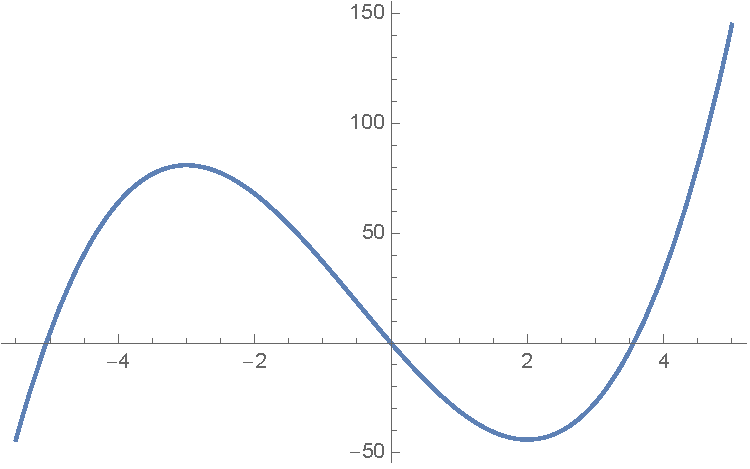
\includegraphics[scale = 0.6]{ex09.pdf}
        \caption{Exercise 9}
        \label{fig:ex09}
      \end{figure}
      
    \newpage

    \item[11]
      \begin{align*}
        f'(x)  & = 4x^3 - 4x \\
        f''(x) & = 12x^2 - 4 \\
      \end{align*}

      \begin{enumerate}[(a)]
        \item $f$ is increasing on $(-1, 0) \cup (1, \infty)$

        \item there is a local maximum at $(0, 3)$ and local minimums at
          $(-1, 2)$ and $(1, 2)$.

        \item $f$ is concave down on $\left( -\frac{\sqrt{3}}{3}, \frac{\sqrt{3}}{3} \right)$ with
          inflection points at $\left( -\frac{\sqrt{3}}{3}, \frac{22}{9} \right)$ and
          $\left( \frac{\sqrt{3}}{3}, \frac{22}{9} \right)$.

      \end{enumerate}

      \begin{figure}[H]
        \centering
        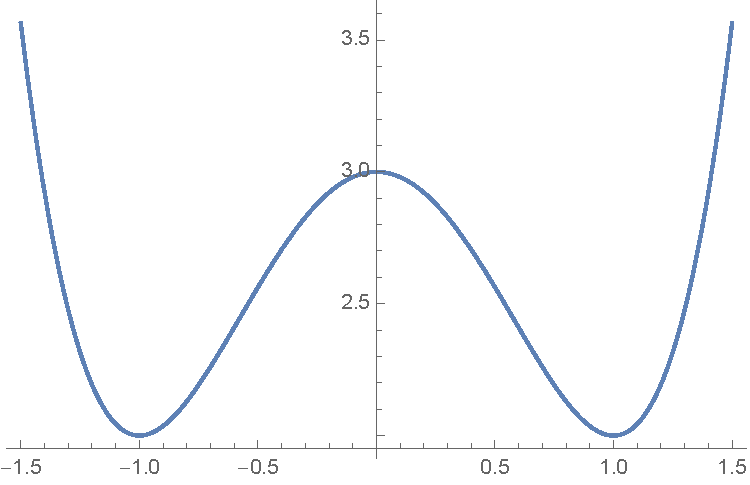
\includegraphics[scale = 0.6]{ex11.pdf}
        \caption{Exercise 11}
        \label{fig:ex11}
      \end{figure}

    \newpage

    % \item[12]
    %   \begin{align*}
    %     f'(x)  & = \frac{6x}{\left(x^2 + 3\right)^2} \\
    %     f''(x) & = - \frac{18 \left(x^2 - 1\right)}{\left(x^2 + 3\right)^3} \\
    %   \end{align*}

    %   \begin{enumerate}[(a)]
    %     \item $f$ is increasing on $(0, \infty)$

    %     \item there is a local minimums at $(0, 0)$ 

    %     \item $f$ is concave down on $\left( -\frac{\sqrt{3}}{3}, \frac{\sqrt{3}}{3} \right)$ 
          
    %       There are inflection points at $\left( -1, \frac{1}{4} \right)$ and 
    %       $\left( 1, \frac{1}{4} \right)$

    %   \end{enumerate}

    %   \begin{figure}[H]
    %     \centering
    %     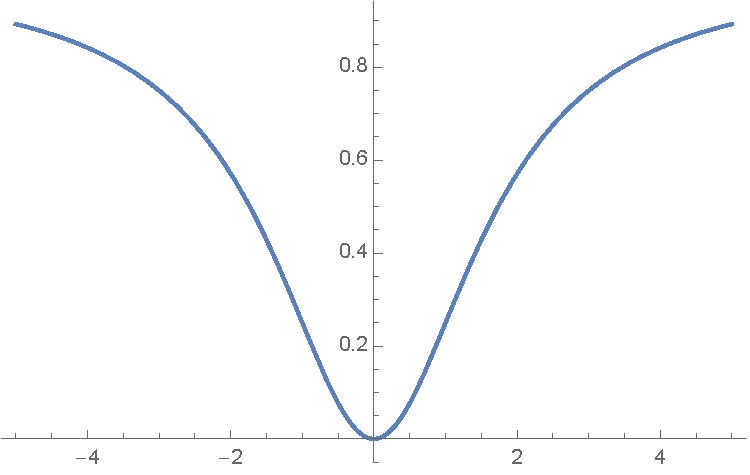
\includegraphics[scale = 0.6]{ex12.pdf}
    %     \caption{Exercise 12}
    %     \label{fig:ex12}
    %   \end{figure}

    \newpage

    \item[33]
      \begin{align*}
        f'(x)  & = 6x^2 - 6x - 12 \\
        f''(x) & = 12x - 6 \\
      \end{align*}

      \begin{enumerate}[(a)]
        \item $f$ is increasing on $(-\infty, -1) \cup (2, \infty)$

        \item there is a local minimum at $(2, -20)$ 

        \item $f$ is concave up on $\left( \frac{1}{2}, \infty \right)$ 
          
          There is an inflection point at $\left( \frac{1}{2}, - \frac{13}{2} \right)$ 

      \end{enumerate}

      \begin{figure}[H]
        \centering
        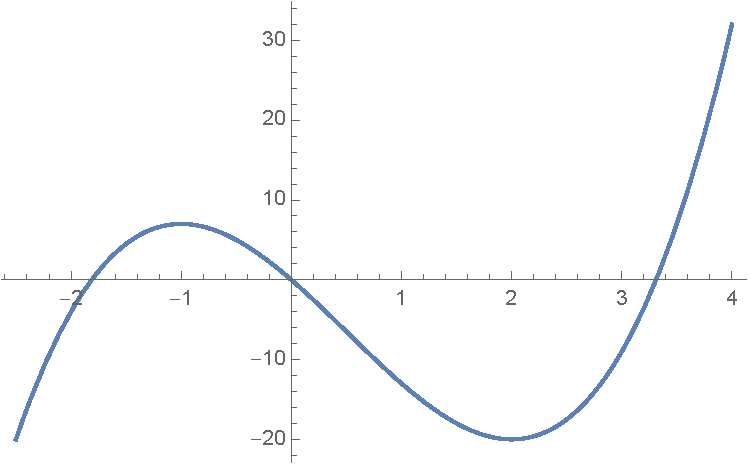
\includegraphics[scale = 0.6]{ex33.pdf}
        \caption{Exercise 33}
        \label{fig:ex33}
      \end{figure}

    \newpage

    \item[34]
      \begin{align*}
        f'(x)  & = 3 - 3x^2 \\
        f''(x) & = -6x \\
      \end{align*}

      \begin{enumerate}[(a)]
        \item $f$ is increasing on $(-1, 1)$

        \item There is a local minimum at $(-1, 0)$ 

        \item $f$ is concave up on $\left( -\infty, 0 \right)$ 
          
          There is an inflection point at $(0, 2)$ 

      \end{enumerate}

      \begin{figure}[H]
        \centering
        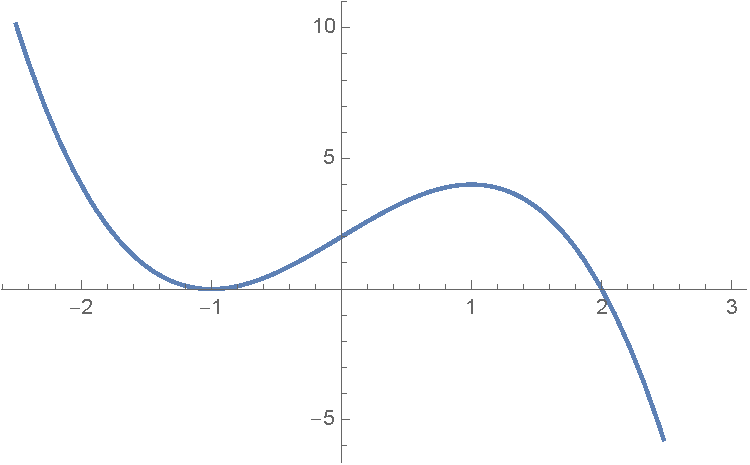
\includegraphics[scale = 0.6]{ex34.pdf}
        \caption{Exercise 34}
        \label{fig:ex34}
      \end{figure}

    \newpage

    \item[35]
      \begin{align*}
        f'(x)  & = 4x - 4x^3 \\
        f''(x) & = 4 - 12x^2 \\
      \end{align*}

      \begin{enumerate}[(a)]
        \item $f$ is increasing on $(-\infty, -1) \cup (0, 1)$

        \item there is a local minimums at $(0, 2)$ 

        \item $f$ is concave up on $\left( -\frac{\sqrt{3}}{3}, \frac{\sqrt{3}}{3} \right)$ 
          
          There are inflection points at $\left( -\frac{\sqrt{3}}{3}, \frac{23}{9} \right)$ and 
          $\left( \frac{\sqrt{3}}{3}, \frac{23}{9} \right)$

      \end{enumerate}

      \begin{figure}[H]
        \centering
        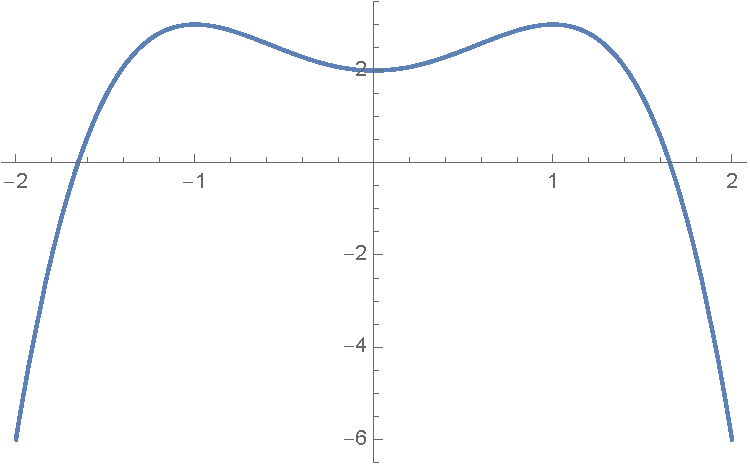
\includegraphics[scale = 0.6]{ex35.pdf}
        \caption{Exercise 35}
        \label{fig:ex35}
      \end{figure}

    \newpage

    \item[39]
      \begin{align*}
        f'(x)  & = \frac{3x + 6}{2 (x + 1)^{1/2}} \\
        f''(x) & = \frac{3x + 12}{4 (x + 1)^{3/2}} \\
      \end{align*}

      \begin{enumerate}[(a)]
        \item $f$ is increasing on $(-2, \infty)$

        \item there is a local minimum at $(-2, -2)$ 

        \item $f$ is concave up for all points in the domain: $(-3, \infty)$

      \end{enumerate}

      \begin{figure}[H]
        \centering
        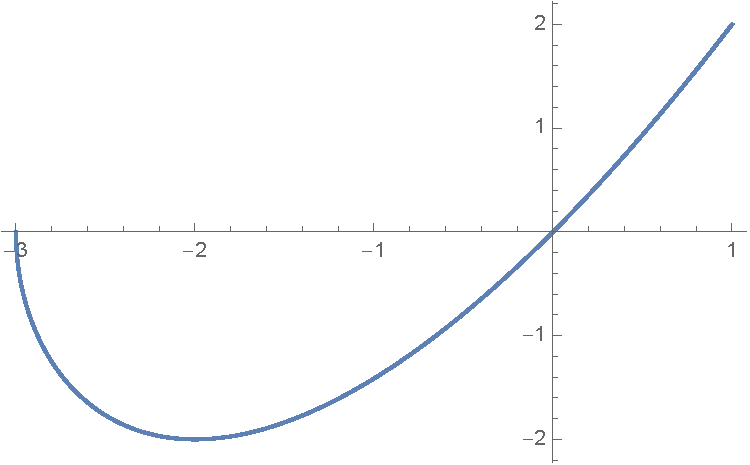
\includegraphics[scale = 0.6]{ex39.pdf}
        \caption{Exercise 39}
        \label{fig:ex39}
      \end{figure}

    \newpage

    \item[40]
      \begin{align*}
        f'(x)  & = -1 + 2x^{-1/3} \\
        f''(x) & = -\frac{2}{3} x^{-4/3} \\
      \end{align*}

      \begin{enumerate}[(a)]
        \item $f$ is increasing on $(0, 8)$

        \item there is a local maximum at $(8, 4)$ 

        \item $f$ is concave down for all points in the domain: $(0, \infty)$

      \end{enumerate}

      \begin{figure}[H]
        \centering
        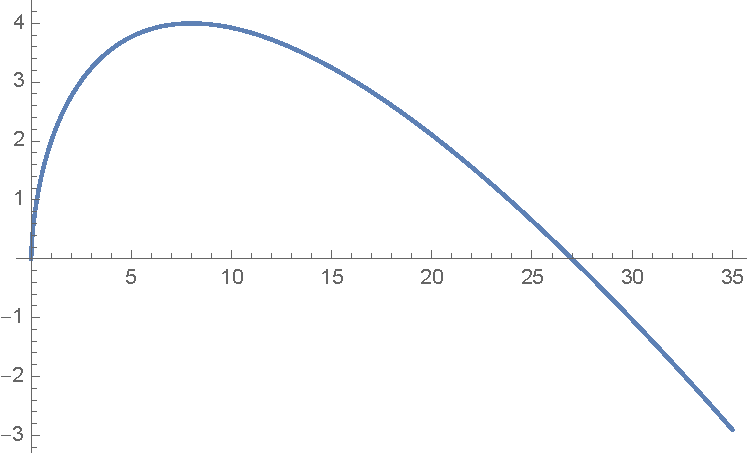
\includegraphics[scale = 0.6]{ex40.pdf}
        \caption{Exercise 40}
        \label{fig:ex40}
      \end{figure}

  \end{description}

  \newpage

  \section{Section 4.7} % (fold)

  \begin{description}
    \item[7]
      \begin{align*}
        \frac{dY}{dN} &= \frac{ k \left( 1 - N^2 \right) }{ \left( N^2 + 1\right )^2 }
        \\
        1 - N^2 & = 0 \\
        N       & = \boxed{ 1 } \\
      \end{align*}

    \item[11]
      If $x$ is the length of side with the middle division and $y$ is the length of the other side,
      we want to minimize the total fence used:

      Find an equation for the perimeter in terms of the length of one of the sides:
      \begin{align*}
        xy & = \frac{3}{2} \\
        y  & = \frac{3}{2} x^{-1} \\
        \\
        P & = 3x + 2y \\
        P & = 3x + 3x^{-1} \\
      \end{align*}

      Minimize the perimeter length:
      \begin{align*}
        P'          & = 3 - 3x^{-2} \\
        3 - 3x^{-2} & = 0 \\
        x           & = 1 \\
        \\
        x  & = \boxed{ \unit[1 \times 10^6]{ft} } \\
        y  & = \boxed{ \unit[1.5 \times 10^6]{ft} } \\
      \end{align*}

      The best shape is a rectangle with the long side 1.5 million feet and the short side 1 million
      feet, with the extra fence parallel to the short side.

    \item[21]
      The relationship between the sides and the radius is:
      \begin{align*}
        x^2 + y^2 & = (2r)^2 \\
        y         & = \sqrt{4r^2 - x^2} \\
      \end{align*}

      The area is:
      \[
        A(x) = x (4r^2 - x^2)^{1/2}
      \]

      Find the maximum:
      \begin{align*}
        A(x)          & = x (4r^2 - x^2)^{1/2} \\
        \frac{dA}{dx} & = \frac{4r^2 - 2x^2}{\sqrt{4r^2 - x^2}} \\
        \\
        4r^2 - 2x^2 & = 0 \\
        x           & = r \sqrt{2} \\
        y           & = \sqrt{4r^2 - 2r^2} \\
                    & = r \sqrt{2} \\
      \end{align*}

      \fbox{ The best shape is a square, with side length $r \sqrt{2}$. } 

    \newpage

    \item[38]
      Find an expression for the height in terms of the radius:
      \begin{align*}
        V  & = \frac{1}{3} \pi r^2 h \\
        27 & = \frac{1}{3} \pi r^2 h \\
        h  & = \frac{81}{\pi r^2} \\
      \end{align*}

      The amount of paper used is the surface area:
      \begin{align*}
        A                     & = \pi r \left( r^2 + h^2 \right)^{1/2} \\
        A(r)                  & = \pi r \left( r^2 + \frac{81^2}{\pi^2} r^{-4} \right)^{1/2} \\
                              & \approx \pi r \left( r^2 + 664.768 r^{-4} \right)^{1/2} \\
        \\
        A'(r)                 & \approx \frac{6.28319 r^6 - 2088.43}{r^4 \sqrt{r^2 + 664.768 r^{ - 4}}} \\
        6.28319 r^6 - 2088.43 & = 0 \\
        r                     & \approx \boxed{ \unit[2.63192]{cm} } \\
        h                     & \approx \boxed{ \unit[3.72211]{cm} } \\
      \end{align*}

  \end{description}

  \else
    \vspace{10 cm}
    \begin{quote}
      \begin{em}
        Basically It's a hypocritical view, because what you're saying is it's
        okay for us to live in the dirt, in the gutter, in less than human
        conditions, but it's not okay for us to tell people that we are living
        in these conditions.
      \end{em}
    \end{quote}
    \hspace{2 cm} --Tupac Shakur
  \fi

\end{document}

